% Advisor walkthrough of docs/model-draft.tex: the population model for
% published cohort statistics.
%
% Compile:  cd docs/slides && make          (or: latexmk -pdf model-draft-slides.tex)
% Figures:  figures/*.tex, each standalone.
%
\documentclass[10pt,aspectratio=169]{beamer}

\usetheme{metropolis}
\metroset{numbering=fraction}
\setbeamertemplate{frametitle continuation}{}
\usepackage{appendixnumberbeamer}

\usepackage{amsmath,amssymb}
\usepackage{booktabs}
\usepackage{array}
\usepackage{tabularx}
\usepackage{graphicx}
\usepackage{tikz}
\usetikzlibrary{arrows.meta,positioning}
\graphicspath{{figures/}}

% Same palette as the figures.
\definecolor{popcol}{HTML}{3B4AA6}
\definecolor{mechcol}{HTML}{2E7D5B}
\definecolor{msrcol}{HTML}{EB811B}
\definecolor{datacol}{HTML}{8C3B4A}
\newcommand{\mech}[1]{\textcolor{mechcol}{#1}}
\newcommand{\msr}[1]{\textcolor{msrcol}{#1}}

\newcommand{\Ncal}{\mathcal{N}}
\newcommand{\Mset}{\mathcal{M}}
\newcommand{\Dset}{\mathcal{D}}
\newcommand{\Rset}{\mathcal{R}}
\newcommand{\Bset}{\mathcal{B}}
\newcommand{\Tr}{^{\!\top}}
\DeclareMathOperator{\diag}{diag}
\DeclareMathOperator*{\Cov}{Cov}

% Ragged fixed-width column, width as a fraction of \textwidth.
\newcolumntype{L}[1]{>{\raggedright\arraybackslash}p{#1\textwidth}}

% Grey row label on the two reference slides.
\newcommand{\lab}[1]{{\scriptsize\color{gray}#1}}

% A short line sitting under a figure.
\newcommand{\undercap}[1]{\vspace{-0.2em}{\small\raggedright #1\par}}

% A term, the first time it is used.
\newcommand{\term}[1]{\alert{\textbf{#1}}}

\title{Model-based Meta Analysis in QSP, as an alternative method for producing virtual populations}
\author{Joel Eliason}
\date{\today}

\begin{document}

\maketitle

% ================================================================ motivation
\begin{frame}[t]{What we want, and what gets built}
  In QSP, when we are producing virtual populations, implicitly what we want is the distribution $F$ of the model's parameters across real patients:
  \[ \theta_i \;\sim\; F . \], where each $\theta_i$ represents a virtual patient.

  Everything we would want to report is computed from $F$. What fraction
  respond, how wide the response is, where the tail sits.
  \vfill
  Classically, a \term{virtual population} is not that. It is a fixed set of candidate
  patients (that is, draws $\theta_i$) with weights on them, chosen so that summaries computed from the
  weighted set match the summaries papers printed. So we are still estimating $F$ in a sense, but heuristically.
\end{frame}

\begin{frame}[t]{Why that is a stand-in}
  \[
    \mathcal{P} \;=\; \big\{\ \text{weightings } p \ :\ T(p) = \widehat T\ \big\}
  \]
  \begin{itemize}\setlength\itemsep{10pt}
    \item About 50 published numbers against about $10{,}000$ candidate
      patients, so $\mathcal{P}$ is enormous.
    \item The tie is broken towards the distribution the cloud was drawn from,
      which was made wide on purpose so the cloud would cover everything. Silent
      directions therefore come back that wide, which is wider than anyone
      believes.
    \item One point of $\mathcal{P}$ comes back, with no way to tell which
      directions the data pinned and which that starting distribution did.
  \end{itemize}
  \vfill
  {\small Regularizing (falling back to a default) is not bad -  we do it too. The objection is
   \emph{which} prior, and what comes back.\par}
\end{frame}

\begin{frame}[t]{What this model does instead}
  Put $F$ in a family, and put a posterior on the family:
  \[ \theta_i \mid \phi \;\sim\; F(\cdot\mid\phi), \qquad p(\phi\mid\Dset) . \]
  \begin{itemize}\setlength\itemsep{10pt}
    \item The unknown is $\phi$, a few hundred numbers, rather than a weighting
      on ten thousand patients.
    \item Each posterior draw $\phi^{(t)}$ is an entire population
      $F(\cdot\mid\phi^{(t)})$.
    \item The trade we make is that $F$ has to lie in the family, and we pick the family
      by hand.
  \end{itemize}
  \vfill
  The work is all in $p(\phi\mid\Dset)$, because of what $\Dset$ is.
\end{frame}

\begin{frame}[t]{The problem: what $\Dset$ is}
  \vspace{-0.3em}
  \[ \widehat T \;=\; T\big(\hat F\big) \]
  \vspace{-1.1em}
  \begin{center}\small
  \begin{tabularx}{0.88\textwidth}{@{}lX@{}}
    $\hat F$ & the $n_c\approx 10$ patients a paper had \\
    $T$ & the summary it computed, such as a median or quartile \\
    $\widehat T$ & the number it printed. We have about 54 of them \\
  \end{tabularx}
  \end{center}
  \vspace{-0.2em}
  \begin{center}
    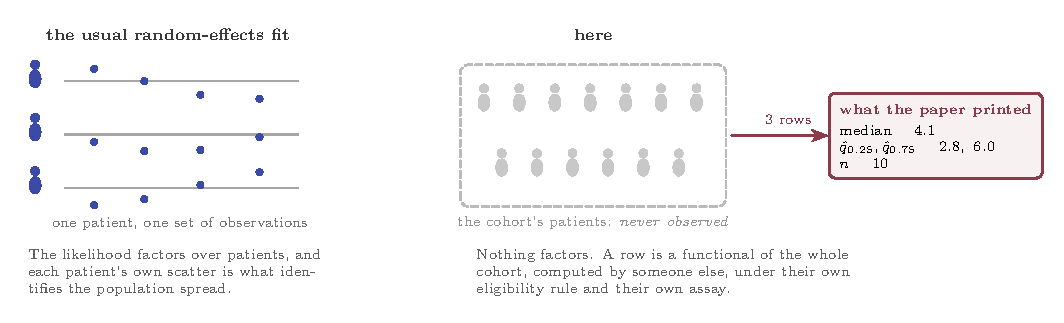
\includegraphics[width=0.84\textwidth]{why_hard.pdf}
  \end{center}
\end{frame}

\begin{frame}[t]{Where this fit sits}
  \begin{center}
    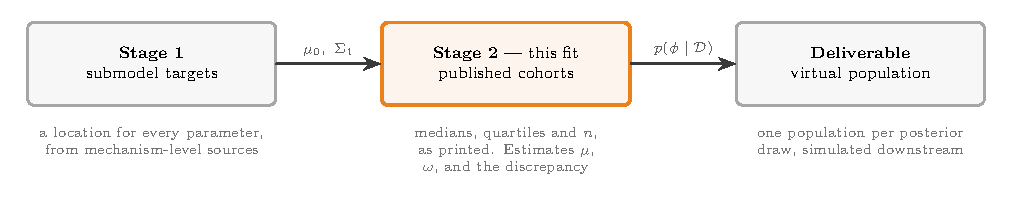
\includegraphics[width=0.96\textwidth]{where_this_sits.pdf}
  \end{center}
  \vfill
  \begin{itemize}\setlength\itemsep{7pt}
    \item \term{Stage 1} already fixed roughly where each of the few hundred
      parameters sits. It says nothing about how much patients differ from one
      another, because its sources are not populations (typically in vitro experiments).
    \item This fit adds that spread, and lets the published cohorts move the
      center as well.
  \end{itemize}
\end{frame}

\begin{frame}[t]{What one paper gives us}
  A paper biopsies ten patients on day 21 and reports the density of CD8$^+$
  T cells in viable tumour, as a median and two quartiles.
  \vspace{0.4em}
  \begin{columns}[T]
    \begin{column}{0.33\textwidth}
      \begin{center}\small
      \begin{tabular}{@{}lr@{}}
        \toprule
        median & $4.1$ \\
        lower quartile & $2.8$ \\
        upper quartile & $6.0$ \\
        \midrule
        patients & $10$ \\
        \bottomrule
      \end{tabular}
      \end{center}
    \end{column}
    \begin{column}{0.62\textwidth}
      Counted the way this model counts them, that is \term{three rows} of data
      rather than one. The whole dataset is about 54 rows, scraped from a wide variety of papers with MAPLE
      \vspace{0.5em}

      This demonstrates the dimensionality differences: Three numbers off ten people, and from roughly fifty such triples we are
      trying to recover a few hundred parameters and how much each of them
      varies between patients.
    \end{column}
  \end{columns}
\end{frame}

\begin{frame}[t]{Some vocabulary}
  \begin{block}{}
    \begin{tabularx}{\textwidth}{@{}lX@{}}
      \textbf{readout} & the quantity a paper reports. Here, the density of
        killer T cells. \\[5pt]
      \textbf{cohort} & the group of patients it was reported on, with its own
        size and its own rule about who was allowed in. \\[5pt]
      \textbf{row} & one readout, from one cohort, summarized one way. The
        median above is a row, and each quartile is another. \\[5pt]
      \textbf{scenario} & the situation the simulator is run in so that it
        matches the cohort: untreated, say, or three weeks into treatment. \\[5pt]
      \textbf{block} & a set of cohorts that have to be handled together,
        because they were measured on overlapping patients. \\
    \end{tabularx}
  \end{block}
\end{frame}

% ---------------------------------------------------------------- how others do it
\begin{frame}[t]{How virtual populations get built: a comparison of methods}
  \vspace{-0.4em}
  \begin{center}
    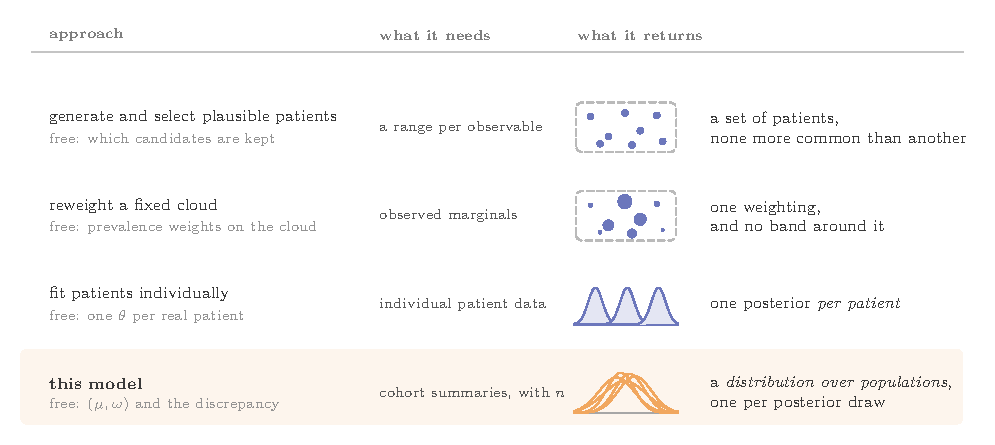
\includegraphics[width=0.95\textwidth]{landscape.pdf}
  \end{center}
  \vspace{-0.3em}
  {\scriptsize\raggedright Cheng et al.\ 2017 (QSP Toolbox); Rieger et al.\ 2018;
   Allen, Rieger \& Musante 2016; Paul et al.\ 2024. Row two is
   \texttt{vpop/weighting.py}.\par}
\end{frame}

\begin{frame}[t]{Deeper into the second method (Allen/Rieger)}
  The first and second rows are the standard methods in this field. In particular, the second works like this:
  \begin{center}
    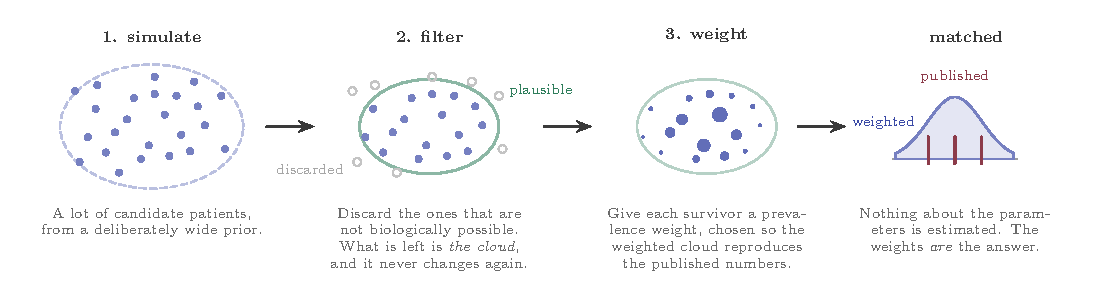
\includegraphics[width=\textwidth]{fixed_cloud.pdf}
  \end{center}
  \vfill
  The parameter values are settled at step two and never touched again. All the
  data decide is how common each of those already-chosen patients is.
\end{frame}

% \begin{frame}[t]{The same picture, twice}
%   \begin{center}
%     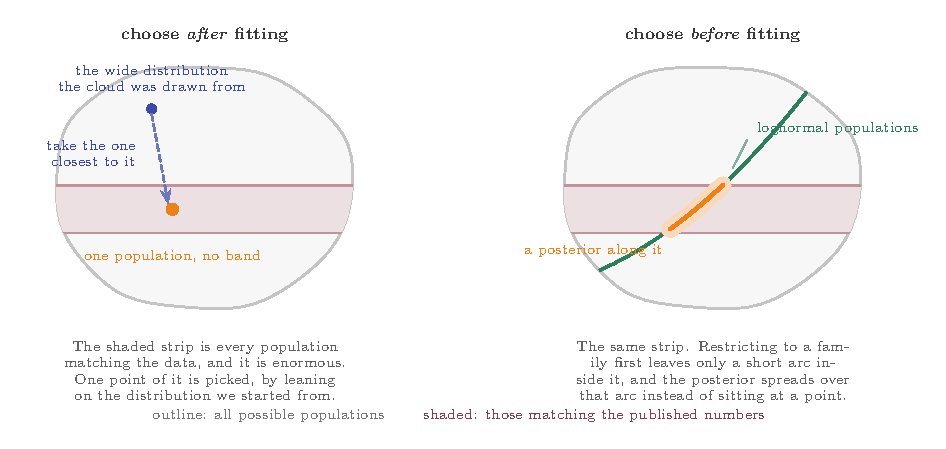
\includegraphics[height=0.66\textheight]{regularize_when.pdf}
%   \end{center}
%   \undercap{Both narrow the answer down. The difference is when, and only
%     narrowing it beforehand leaves something a posterior can be spread over.}
% \end{frame}

\begin{frame}[t]{Diagnostics from this method}
  \[ \mathrm{ESS} \;=\; \Big(\textstyle\sum_m p_m^2\Big)^{-1} \]
  In my experience fitting this on the PDAC model, this collapses. A handful of the $10{,}000$ candidates end up
  carrying nearly all the mass, and there are two reasons for it.
  \begin{itemize}\setlength\itemsep{10pt}
    \item \textbf{Dimension.} One weight vector has to satisfy every readout at
      once, and the feasible fraction of the cloud shrinks with the number of
      readouts even when the model is right.
    \item \textbf{Miscalibration.} The model cannot reproduce the readouts
      jointly, so the only survivors are cloud members out in the tail.
  \end{itemize}
  \vfill
  These call for opposite remedies: a bigger cloud or a better model.
\end{frame}

% ---------------------------------------------------------------- what is hard
\begin{frame}[t]{What a likelihood needs}
  \[ \widehat T \;\sim\; \Ncal\big(\tau(\phi),\ V\big) \]
  $\tau(\phi)$ is the model's prediction of the printed number, and $V$ sets the (co)variation in $\tau$.
  \vfill
  Four nuances/challenges about this likelihood, in the order the rest of the talk takes them:
  \begin{enumerate}\setlength\itemsep{4pt}\small
    \item $\tau$, the model's prediction, is not the population quantity. That
      median came off ten patients, so we predict the average of a ten-patient
      median - so somehow we have to link from the sample quantity to the population quantity.
    \item Nothing hands us $V$. Papers report spreads, not the uncertainty in
      their own summaries, so the model has to predict $V$ from its own
      patients.
    \item Not all of the bias $\widehat T - \tau$ is biology. Some is the assay and some
      the simulator, and both need somewhere to go other than $\mu$ and $\omega$ - otherwise those parameters end up absorbing technical data issues.
    \item The rows are not independent. One paper reports several numbers off
      the same patients, so $V$ is block diagonal - capturing that numbers reported from the same study (typically) come from the same patients.
  \end{enumerate}
\end{frame}

\begin{frame}[t]{First: ten patients do not have the population's median}
  \[
    \tau \;=\; T\big(\tilde F\big)
    \qquad\text{versus}\qquad
    \tau \;=\; \mathbb{E}\big[\,T\big(\tilde F^{\,\ast}\big)\,\big],
    \quad \tilde F^{\,\ast} \text{ an } n_c\text{-sample from } \tilde F .
  \]
  The model has to do what the paper did: take $n_c$ of its own patients,
  compute their median, and average that over draws. This captures the generative process at work here - a patient sample comes from a larger population, which is what we are trying to estimate
  \vfill
  Sample quartiles are biased inward, at both ends, so a printed pair is
  narrower than the population it came from. If we predict population quartiles
  against it, the model looks too wide.

\end{frame}

\begin{frame}[t]{Second: a spread is not an error bar}
  \[ \widehat T \;\sim\; \Ncal\big(\tau(\phi),\ V\big), \qquad V = \ ? \]
  Papers report spreads readily enough. An IQR says how much patients vary; it
  does not say how far the median would move with a different ten. So the model
  predicts $V$ by resampling its own cohort:
  \[ V^{\text{boot}} \;=\; \Cov_{\ast}\big[\,T\big(\tilde F^{\,\ast}\big)\,\big] . \]
  \vfill
  But $\tilde F$ depends on $\phi$. So $V$ is built once at a preliminary
  $\phi_0$ and then frozen, and the fit cannot chase its own error bars.
  \vfill
  What remains is a dependence on $\phi_0$. It is allowable because $V$ only
  weights the residuals: any fixed choice leaves the solution in the right
  place, so $\phi_0$ costs precision and not correctness.
\end{frame}

\begin{frame}[t]{Third: some of the disagreement is not biology}
  \[
    \tau\big(\underbrace{\mu,\omega}_{\text{what we want}}\big)
    \qquad\text{versus}\qquad
    \tau\big(\underbrace{\mu,\omega}_{\text{what we want}},\
      \underbrace{a,\,b,\,\beta}_{\text{assay, simulator}}\big)
  \]
  Two labs with different equipment do not report the same number, and the
  simulator is wrong somewhere as well.
  \vfill
  With no term for it, that disagreement goes into $\mu$ and $\omega$. With one,
  $a$, $b$ and $\beta$ can absorb real biology just as easily as an artefact.
\end{frame}

\begin{frame}[t]{Fourth: the rows are not independent}
  \[
    \prod_{k=1}^{K}\Ncal\big(\widehat T_k;\ \tau_k,\ V_{kk}\big)
    \qquad\text{versus}\qquad
    \prod_{B\in\Bset}\Ncal_{K_B}\big(\widehat T_B;\ \tau_B,\ V_B\big)
  \]
  About 54 rows, and one paper supplies 20 of them off roughly ten patients per
  arm. The left product counts those ten people twenty times.
  \vfill
  So the unit of independence is neither the row nor the cohort. It is the
  \term{block}: cohorts that have to be handled together, either because one row
  is computed from several of them or because they overlap in patients.
\end{frame}

% ================================================================ the model
\begin{frame}[standout]
  The generative model
\end{frame}

\begin{frame}[t]{The chain, end to end}
  \begin{center}
    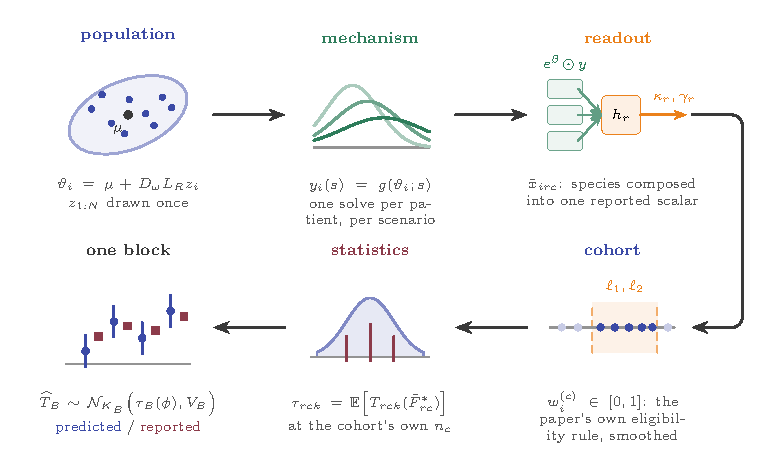
\includegraphics[height=0.70\textheight]{generative_chain.pdf}
  \end{center}
  \undercap{Everything between the ends is deterministic given the fixed cloud
    $z_{1:N}$. The only stochastic step is the last one.}
\end{frame}

\begin{frame}[t]{The whole model: parameters to a row}
  \begingroup\small
  \begin{center}
  \begin{tabular}{@{}r@{\ \ }l@{}}
    \lab{population} & $\vartheta_i = \mu + D_\omega L_R z_i$,\ \ $z_{1:N}$ drawn once \\[5pt]
    \lab{mechanism} & $y_i(s) = g(\vartheta_i;s)$ \\[5pt]
    \lab{readout} & $x_{irc} = h_r\big(y_i(1),\dots,y_i(S)\big)$ \\[5pt]
    \lab{discrepancy} & $\tilde x_{irc}
      = \kappa_r\big(h_r(e^{\beta}\!\odot y_i(s(c))) - c_{rc}\big) + c_{rc} + \gamma_r$ \\[1pt]
     & \lab{with}\ \ $\gamma_r = Z_r\Tr a$,\ \ $\log\kappa_r = Z_r\Tr b$ \\[5pt]
    \lab{eligibility} & $w^{(c)}_i
      = \sigma\big((\tilde x_{irc}-\ell_1)/h_w\big)\,
        \sigma\big((\ell_2-\tilde x_{irc})/h_w\big)$ \\[5pt]
    \lab{statistic} & $\tau_{rck}(\phi)
      = \mathbb{E}\big[T_{rck}(\tilde F^{\,\ast}_{rc})\big]$,\ \
      $\tilde F^{\,\ast}_{rc}$ an $n_c$-sample from $\tilde F_{rc}$ \\[5pt]
    \lab{observation} & $\widehat T_B \sim \Ncal_{K_B}\big(\tau_B(\phi),V_B\big)$,\ \
      independent across blocks \\[5pt]
    \lab{study effect} & $\eta_s \sim \Ncal(0,\tau_\eta^2)$ on study $s$'s
      location rows, marginalised into $V_B$ \\[5pt]
    \lab{error bars} & $V_B = V^{\text{boot}}_B + E_B
      + \tau_\eta^2\sum_s \mathbf{1}^{\mathrm{loc}}_{B,s}\mathbf{1}^{\mathrm{loc}\Tr}_{B,s}$,\ \
      built at $\phi_0$ and frozen \\
  \end{tabular}
  \end{center}
  \endgroup
  \vfill
  {\small Here first, so the shape is visible. Each line gets its own slide after
   this.\par}
\end{frame}

\begin{frame}[t]{The whole model: priors, posterior, deliverable}
  \begingroup\small
  \begin{center}
  \begin{tabular}{@{}r@{\ \ }l@{}}
    \lab{centre} & $\mu \sim \Ncal_P(\mu_0,\Sigma_1)$,\ \ from stage 1 \\[5pt]
    \lab{spread} & $\log\omega_j = \log\omega_{0j} + s + u_j$,\ \
      $\textstyle\sum_{j\notin\Mset} u_j = 0$,\ \ $\omega_0$ elicited by role \\[5pt]
    \lab{correlation} & $R = \Lambda\Lambda\Tr + \diag(\psi^2)$,\ \ $\Lambda$ elicited \\[5pt]
    \lab{assay} & $a \sim \Ncal(0,\sigma_a^2 I)$,\ \ $b \sim \Ncal(0,\sigma_b^2 I)$ \\[5pt]
    \lab{species} & $\beta_q = \tau_\beta\big(\beta^{\text{raw}}_q - \bar\beta^{\text{raw}}\big)$,\ \
      $\tau_\beta$ fixed \\[5pt]
    \lab{conversions} & $\log R_m \sim \Ncal\big(\log R_{0m},\sigma_{Rm}^2\big)$ \\[9pt]
    \lab{unknowns} & $\phi = \big(\mu,\ s,\ u^{\text{raw}},\ \log\omega_{\Mset},\
      a,\ b,\ \beta^{\text{raw}}_{\mathcal{S}},\ \log R_{\mathcal{A}}\big)$ \\[5pt]
    \lab{posterior} & $p(\phi\mid\Dset) \propto p(\phi)\prod_{B\in\Bset}
      \Ncal\big(\widehat T_B;\tau_B(\phi),V_B\big)$ \\[5pt]
    \lab{deliverable} & $p(\theta_{\text{new}}\mid\Dset)
      = \int \Ncal_P\big(\log\theta_{\text{new}};\mu,\Omega\big)\,p(\phi\mid\Dset)\,d\phi$ \\
  \end{tabular}
  \end{center}
  \endgroup
  \vfill
  {\small Above the gap, what we bring to the problem. Below it, what we solve
   for and what comes out.\par}
\end{frame}

\begin{frame}[t]{Population}
  A patient is a parameter vector. The population is a lognormal over them:
  \[
    \vartheta_i \mid \mu,\omega \sim \Ncal_P(\mu,\Omega),
    \qquad \Omega = D_\omega R D_\omega,
    \qquad \vartheta = \log\theta ,
  \]
  with $\mu$ the centre and $\omega$ the spread of each parameter. $\omega$ sets
  the marginals; $R$ sets everything joint.
  \vfill
  $R$ is not fitted: about 50 rows cannot inform $P(P-1)/2$ correlations. It is
  \alert{elicited}, and deliberately not inherited from stage 1.
  \begin{itemize}\small\setlength\itemsep{5pt}
    \item A stage-1 posterior correlation is epistemic: the same data constrained
      those two jointly. Reading it here asserts something else and unevidenced,
      that a patient high in one is high in the other.
    \item So each parameter loads on a few latent patient axes, and $R$ is what
      the shared loadings imply:
      \[ z_{ij} = \textstyle\sum_k \Lambda_{jk}f_{ik} + \psi_j e_{ij},
         \qquad R = \Lambda\Lambda\Tr + \diag(\psi^2). \]
  \end{itemize}
\end{frame}

\begin{frame}[t]{Two elicited inputs, one form}
  Nothing measures a between-patient spread, and nothing measures a
  between-patient correlation. Both are stated as claims about single parameters,
  in bins, each bin named for its \term{warrant} rather than its value.
  \vspace{0.2em}
  \begin{columns}[t]
    \begin{column}{0.53\textwidth}
      {\small\textbf{Role}: how wide, $\to \omega_0$\par}
      \begin{center}\scriptsize
      \begin{tabular}{@{}lrr@{}}
        \toprule
        & $\omega_0$ & \# \\
        \midrule
        \texttt{patient\_trait} & $0.70$ & $18$ \\
        \texttt{lumped} & $0.50$ & $50$ \\
        \texttt{default} & $0.35$ & $3$ \\
        \texttt{packing\_limit} & $0.15$ & $12$ \\
        \texttt{material\_constant} & $0.10$ & $4$ \\
        \texttt{structural} & $0.05$ & $15$ \\
        \bottomrule
      \end{tabular}
      \end{center}
    \end{column}
    \begin{column}{0.43\textwidth}
      {\small\textbf{Loading}: what it varies with, $\to \Lambda$\par}
      \begin{center}\scriptsize
      \begin{tabular}{@{}lrr@{}}
        \toprule
        & $|\Lambda_{jk}|$ & explains \\
        \midrule
        \texttt{primary} & $0.8$ & $64\%$ \\
        \texttt{secondary} & $0.5$ & $25\%$ \\
        \texttt{weak} & $0.3$ & $9\%$ \\
        \bottomrule
      \end{tabular}
      \end{center}
      {\scriptsize No declared loading means uncorrelated, and that is the
       default. Communality capped at $0.81$, so $R$ is strictly positive
       definite and no nearest-correlation projection is ever called.\par}
    \end{column}
  \end{columns}
  \vspace{0.2em}
  {\small $O(P)$ claims rather than $P(P-1)/2$. The gaps are load-bearing too:
   $\tau_\omega=0.085$ is a quarter of the narrowest, so the fitted pattern
   cannot move a parameter out of the role it was given.\par}
\end{frame}

\begin{frame}[t]
  We draw $N$ standard normal vectors \emph{once}, at the start, and reuse the
  same ones for every $(\mu,\omega)$ the fit tries:
  \[ \vartheta_i = \mu + D_\omega L_R z_i, \qquad R = L_R L_R\Tr . \]
  \begin{itemize}\setlength\itemsep{8pt}
    \item Redrawing them each time would make the predicted rows jitter, and the
      fit would chase that jitter instead of the parameters.
    \item Reusing them also keeps patient $i$ the same person across scenarios,
      which is what lets a readout compare a patient against themselves.
    \item With hundreds of parameters nothing gradient-free is in reach, so
      every step from $\phi$ to a predicted row needs a derivative. This is the
      first of three places that constraint decides a modelling choice. The
      others are enrolment and the quantile.
  \end{itemize}
\end{frame}

\begin{frame}[t]{Mechanism and readout}
  Simulate patient $i$ under scenario $s$, read the species at the measured
  time, and compose them into the scalar a study reports:
  \[
    y_i(s) = g(\vartheta_i;s) \in \mathbb{R}^Q_+ ,
    \qquad
    x_{irc} = h_r\big(y_i(1),\dots,y_i(S)\big).
  \]
  \begin{itemize}
    \item Most readouts use only $y_i(s(c))$. $h_r$ takes the whole scenario set
      anyway, so that a fold change is a contrast within one patient.
    \item $h_r$ carries the unit conversions, and is already fixed by the target
      definitions.
    \item In the fit, $g$ is a trained emulator $\widehat g$ rather than the
      solver itself. The error that introduces is priced in later.
  \end{itemize}
\end{frame}

% ---------------------------------------------------------------- discrepancy
\begin{frame}[t]{Discrepancy}
  Two terms, separated by where they enter: one on the species, one on the
  finished row.
  \[
    \tilde x_{irc}
    = \msr{\kappa_r}\Big(h_r\big(
      \underbrace{\mech{e^{\beta}}\odot y_i(s(c))}_{\text{upstream of }h_r}
      \big) - c_{rc}\Big) + c_{rc} + \msr{\gamma_r},
    \qquad
    \msr{\gamma_r = Z_r\Tr a}, \quad \msr{\log\kappa_r = Z_r\Tr b}.
  \]
  \begin{itemize}
    \item \mech{$\beta\in\mathbb{R}^Q$} biases each \emph{species} on the log
      scale, shared across readouts and scenarios.
    \item \msr{$a$ and $b$} are the location and scale halves of an affine map on
      the \emph{readout}. $Z_r$ holds assay modality and quantity type.
    \item $\beta=0,a=0,b=0$ is a model biased in neither location nor scale on
      any observed species.
  \end{itemize}
\end{frame}

\begin{frame}[t]{Why the two are separable at all}
  A free offset per row would fit everything and mean nothing. These two are
  earned by where they enter, because that decides how they propagate.
  \begin{itemize}\setlength\itemsep{9pt}
    \item \mech{$\beta$} sits upstream of $h_r$, so the composition carries it: a
      ratio inherits $\beta_{q_1}-\beta_{q_2}$, a percentage inherits
      $\beta_q-\beta_{\mathrm{nuc}}$, a sum inherits a weighted combination.
    \item \msr{$\gamma_r$} sits downstream, so it cannot decompose. It shifts the
      finished number and does nothing else.
    \item One species biased at the source therefore leaves a coordinated
      pattern across every readout that touches it, in ratios the compositions
      fix in advance. A readout-level term cannot produce that pattern.
  \end{itemize}
\end{frame}

\begin{frame}[t]{Where each one enters}
  \begin{center}
    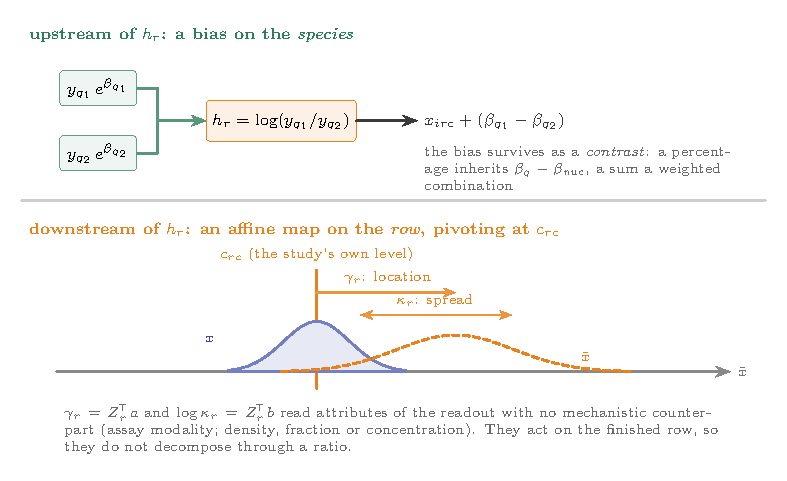
\includegraphics[height=0.80\textheight]{discrepancy.pdf}
  \end{center}
\end{frame}

\begin{frame}[t]{The pivot: what does $\kappa_r$ stretch about?}
  Stretching needs a centre to stretch about. We use $c_{rc}$, the level readout
  $r$ sits at in cohort $c$, computed once from the prior and never fitted.
  \begin{itemize}\setlength\itemsep{8pt}
    \item Stretch about zero instead and $\kappa_r$ moves the readout as well as
      widening it, because a log density sits nowhere near zero. It would be
      doing $\gamma_r$'s job as well as its own.
    \item Stretching about the study's own level keeps them apart: $\kappa_r$ is
      purely spread within the cohort, $\gamma_r$ purely where the cohort sits.
    \item Every cohort gets its own $c_{rc}$, and that costs no parameters,
      because those levels are fixed before the fit starts.
  \end{itemize}
\end{frame}

\begin{frame}[t]{Cohort selection}
  Papers enrol patients on a criterion, so the model has to as well. A rule like
  ``baseline density between $\ell_1$ and $\ell_2$'' becomes a weight between $0$
  and $1$ on each simulated patient, with a logistic $\sigma$ standing in for the
  hard cut-off:
  \[
    w^{(c)}_i = \sigma\!\big((\tilde x_{irc}-\ell_1)/h_w\big)\,
                \sigma\!\big((\ell_2-\tilde x_{irc})/h_w\big).
  \]
  \begin{itemize}
    \item Soft because a hard cut-off has no derivative: one patient crossing the
      line would step the prediction. This is the second of the three.
    \item The rule is written in reported units, so it reads $\tilde x$, the
      value \emph{after} the assay bias. Who is eligible therefore shifts as $a$,
      $b$ and $\beta$ shift. Enrolment is part of the fit, not fixed beforehand.
  \end{itemize}
\end{frame}

% ================================================================ cloud to row
\begin{frame}[standout]
  From a cloud to a row
\end{frame}

\begin{frame}[t]{A paper prints the median of nine patients. What do we predict?}
  \vfill
  Not the population median. The median of nine draws is a random variable, and
  the model has to predict its \emph{mean}:
  \[
    \tau_{rck}(\phi) = \mathbb{E}\Big[\,T_{rck}\big(\tilde F^{\,\ast}_{rc}\big)\Big],
    \qquad \tilde F^{\,\ast}_{rc} = \text{an } n_c\text{-sample from } \tilde F_{rc}.
  \]
  \vfill
  Same functional, same sample size, computed on the model's own predicted
  patients. That expectation is what $\tau$ is: the mean of the row, not the
  population quantity the row is trying to estimate.
\end{frame}

\begin{frame}[t]{Why the distinction is not academic}
  \begin{itemize}\setlength\itemsep{9pt}
    \item Take a population with log-scale spread $1$. Its lower quartile is
      $-0.674$. Draw nine patients from it, and the lower quartile you compute
      averages $-0.570$: pulled towards the middle, and the upper quartile is
      pulled in too.
    \item So a model predicting \emph{population} quartiles can only meet a
      reported pair by shrinking its spread to \alert{$0.845$}. That is a 15\%
      error in the one number this whole fit exists to produce.
    \item The gap closes as the cohort gets bigger, not as the model's own cloud
      gets better, so nothing else in the fit can absorb it.
  \end{itemize}
  \vfill
  The population quantity is still what we deliver. It is read off the posterior
  predictive at the end, not off any row.
\end{frame}

\begin{frame}[t]{And the estimator has to be differentiable}
  \begingroup\small
  \[
    \hat q(p) = \frac{\sum_i k_i x_{(i)}}{\sum_i k_i},
    \qquad k_i = w_{(i)} f_{\mathrm{B}}\big(c_i;\varkappa,n_c-\varkappa+1\big),
    \qquad c_i = \frac{\sum_{l\le i} w_{(l)} - \tfrac12 w_{(i)}}{\sum_l w_l}.
  \]
  \endgroup
  \begin{center}
    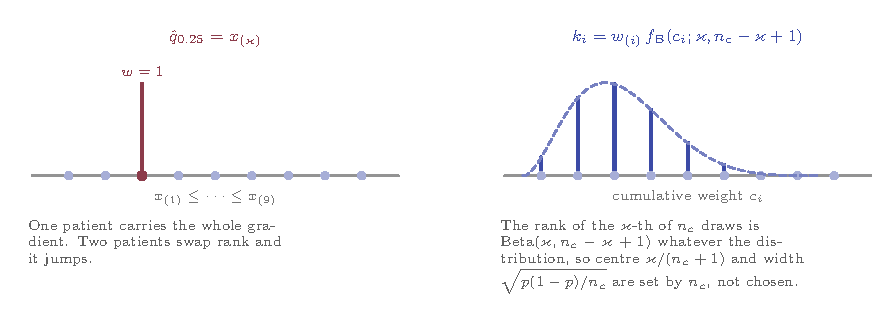
\includegraphics[width=0.60\textwidth]{smooth_quantile.pdf}
  \end{center}
  \vspace{-0.3em}
  {\small\raggedright The rank of the order statistic a cohort's rule points at
   is $\mathrm{Beta}(\varkappa,n_c-\varkappa+1)$ whatever the population is, so
   these weights are not a smoothing knob: they compute exactly the expectation
   above, and differentiability comes free. A width is out of the kernel's reach,
   though. An sd or an IQR is no order statistic, so it enters as its log, and
   that log is what makes $\kappa_r$ an additive shift on the row.\par}
\end{frame}

% ---------------------------------------------------------------- blocks
\begin{frame}[t]{Blocks}
  \begingroup\small
  \[
    \widehat T_B \sim \Ncal_{K_B}\big(\tau_B(\phi),V_B\big),
    \qquad \widehat T_B \perp \widehat T_{B'} \ \text{ for } B\neq B'.
  \]
  \endgroup
  \vspace{-0.5em}
  \begin{center}
    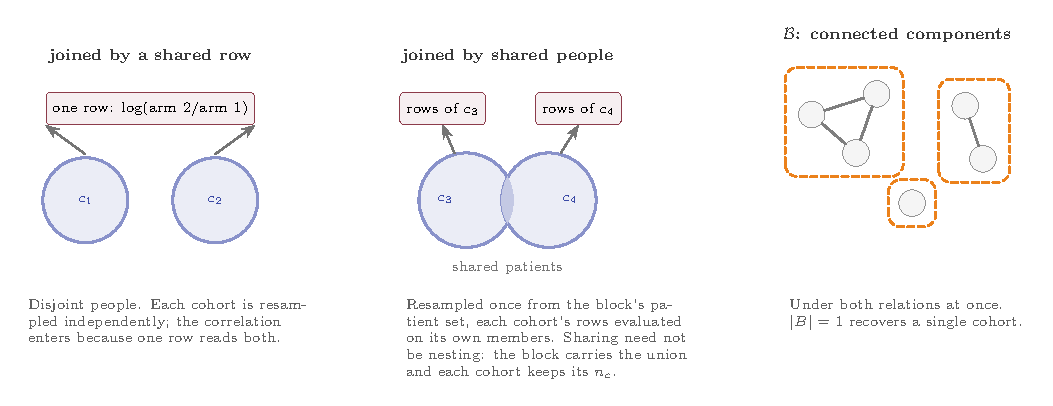
\includegraphics[width=0.70\textwidth]{blocks.pdf}
  \end{center}
  \vspace{-0.2em}
  {\small\raggedright The Gaussian is a working model for a statistic of ten
   patients rather than a derived sampling distribution. What that makes of the
   posterior is an estimating equation, not a likelihood, and it is also why $V$
   is held fixed.\par}
\end{frame}

\begin{frame}[t]{A study is not just its rows}
  Nothing in $\phi$ is indexed by cohort, so two labs reporting the same readout
  at different levels have nowhere to put the difference. Give each study one
  shift on its own location rows:
  \begingroup\small
  \[ \widehat T_B \mid \eta \sim \Ncal\Big(\tau_B(\phi)
       + \textstyle\sum_s \eta_s\,\mathbf{1}^{\mathrm{loc}}_{B,s},\ V_B\Big),
     \qquad \eta_s \sim \Ncal(0,\tau_\eta^2). \]
  Gaussian and additive, so it marginalises exactly:
  \[ \widehat T_B \sim \Ncal\Big(\tau_B(\phi),\ V_B + \tau_\eta^2
       \textstyle\sum_s \mathbf{1}^{\mathrm{loc}}_{B,s}
       \mathbf{1}^{\mathrm{loc}\Tr}_{B,s}\Big). \]
  \endgroup
  \begin{itemize}\small\setlength\itemsep{4pt}
    \item No coordinate added to $\phi$, and the term is free of $\phi$, so $V$
      stays frozen and no $\log\det$ comes back.
    \item \alert{One study supplies 20 of the 55 rows.} Its within-study
      contrasts keep full weight; only their common level is discounted.
    \item $\tau_\eta$ is fixed, not free: 22 studies against 55 rows, 13 of them
      reporting a single row a free shift would fit exactly, and 8 directions
      already spanned by $Z$.
  \end{itemize}
\end{frame}

% ---------------------------------------------------------------- V_B
\begin{frame}[t]{Nobody printed an error bar}
  The observation equation needs $V_B$, and most sources give nothing to build
  one from. So predict it: resample the model's own cohort.
  \[
    V_B = V^{\text{boot}}_B + E_B,
    \qquad
    V^{\text{boot}}_B = \Cov_{\ast}\!\big[T_B(\tilde F^{\ast}_B)\big]_{\phi_0} .
  \]
  \begin{itemize}
    \item Sampling noise from the predicted cloud, emulator error on top.
    \item Built once at a plug-in $\phi_0$, a fixed guess at the answer used only
      to size the error bars, and frozen there.
  \end{itemize}
\end{frame}

\begin{frame}[t]{What drawing whole patients buys}
  \begin{itemize}\setlength\itemsep{9pt}
    \item A resampled patient carries its whole vector $\tilde x_{ic}$. That is
      what moves the dependence between readouts into $V_B$, rather than leaving
      it to be asserted.
    \item Where cohorts of a block share people the draw is common, and that is
      the only source of across-cohort correlation.
    \item Two readouts of one cohort that share a denominator move almost in
      lockstep, which leaves $V_B$ close to singular. A small $\epsilon I$ is
      added before it is inverted.
  \end{itemize}
  \vfill
  The cost of all three: $V_B$ now rests entirely on the predicted cloud.
\end{frame}

\begin{frame}[t]{The guard on that cost}
  A cloud that is too narrow makes every error bar too small, the likelihood
  then overrides the prior, and nothing in the fit catches it. So check first,
  against any source that does report a sampling uncertainty $U_{rck}$:
  \[
    \varrho_{rck} = U_{rck}\Big/\sqrt{\big(V^{\text{boot}}_c\big)_{rck,rck}} .
  \]
  \begin{itemize}
    \item Above one, the predicted cloud is too narrow at that readout.
    \item Computed before fitting, so it is a prior predictive check on exactly
      the rows that now carry $\omega$.
    \item \alert{Fix the model rather than widening $V_B$}: widening hides what
      is being tested.
  \end{itemize}
\end{frame}

\begin{frame}[t]{Emulator error}
  Draw $L$ held-out clouds at $\phi_0$ and evaluate each both ways:
  \[
    d^{(\ell)}_B = \tau^{\widehat g}_B(\phi_0;z^{(\ell)}) - \tau^{g}_B(\phi_0;z^{(\ell)}),
    \qquad E_B = \Cov_\ell\big[d^{(\ell)}_B\big].
  \]
  \begin{itemize}
    \item Defined on the \emph{statistics}, not the readouts: the map from a
      readout error to a statistic error depends on the functional.
    \item A covariance only sees how the error \emph{varies}. If the emulator
      is off by the same amount every time, $E_B$ is blind to it, so
      \alert{report the average error $\bar d_B$ alongside}. The second check
      later asks whether the discrepancy map can absorb it.
  \end{itemize}
\end{frame}

\begin{frame}[t]{Where $\widehat g$ is trained is part of the model}
  $E_B$ and $\bar d_B$ are properties of $\widehat g$, and $\widehat g$ is a
  property of the values it was trained on.
  \begin{itemize}\setlength\itemsep{8pt}
    \item The fit calls it at $\mu + D_\omega L_R z_i$, so the values it will be
      asked about are spread with covariance about $\Sigma_1+\Omega$. Train it on
      a design drawn from that same law, widened at the edges.
    \item \alert{Every parameter has to vary in the design.} Pin one and the
      emulator has never seen it move, so the likelihood along it is not flat,
      it is undefined.
    \item Score it on a fresh draw, not on a held-out slice of the design.
      Space-filling designs are built so their halves interleave, so a split
      would test it on points it effectively already saw.
  \end{itemize}
\end{frame}

\begin{frame}[t]{One number, one job}
  A reported uncertainty could either set the error bar on its row or say
  something about population width. It cannot do both.
  \begin{itemize}
    \item \alert{It always goes to width.} No parameter here has a published
      between-patient spread, so width rows are the only thing that says
      anything about $\omega$. Error bars, by contrast, the bootstrap gives us on
      every row for nothing.
    \item What we predict still depends on which number the paper printed. A
      standard deviation describes the patients; a standard error describes how
      well the study pinned down its own summary. \alert{At $n_c=10$ they differ
      by a factor of $3.2$}, so the extraction has to record which one it is.
    \item Either way the row is worth having, and it does not make the ambiguity
      at the end of the deck any worse.
  \end{itemize}
\end{frame}

% ================================================================ priors
\begin{frame}[standout]
  Priors and posterior
\end{frame}

\begin{frame}[t]{Priors: location and spread}
  \[ \mu \sim \Ncal_P(\mu_0,\Sigma_1) \]
  from the stage-1 composite prior. Write $\Mset$ for the parameters whose
  between-patient spread some source has actually measured; today it is empty.
  For $j\in\Mset$, $\log\omega_j$ concentrates at $\log\omega_{0j}$ with
  precision set by that source's $n_j$. For the rest,
  \[
    \log\omega_j = \log\omega_{0j} + s + u_j,
    \qquad \textstyle\sum_{j\notin\Mset} u_j = 0 .
  \]
  \begin{itemize}\small
    \item $s$ is how much wider the population is overall; $u$ is the pattern
      across parameters.
    \item Without the constraint the two are not separately defined: add a
      constant to $s$, subtract it from every $u_j$, and every $\omega_j$ comes
      out identical. Summing the $u_j$ to zero removes that freedom and leaves
      $s$ as the only overall level.
    \item Worth the trouble: $s$ is the part that reaches the virtual population,
      and the part the last slides are about.
  \end{itemize}
\end{frame}

\begin{frame}[t]{Priors: discrepancy}
  \textbf{Measurement.} Free, because it has no parameter twin:
  \[ a\sim\Ncal(0,\sigma_a^2 I), \qquad b\sim\Ncal(0,\sigma_b^2 I),
     \qquad \sigma_a=\sigma_b=0.5 . \]
  \textbf{Mechanism.} Tightly shrunk, because it competes with $\mu$:
  \[
    \beta_q = \tau_\beta\big(\beta^{\text{raw}}_q - \bar\beta^{\text{raw}}\big),
    \qquad \tau_\beta = 0.15 \ \text{fixed}.
  \]
  for a declared handful of species, by default the shared denominators.
  \begin{itemize}\small
    \item Fixed rather than estimated: estimating $\tau_\beta$ gives the sampler
      a funnel-shaped posterior, which it handles badly, and with $\beta$ centred
      there is too little left for it to learn in exchange.
    \item Centred because otherwise there is an exact alias. Give every species
      the same bias and it cancels out of every ratio and fraction, leaving only
      a shift in the densities, which $\gamma$ already produces. The data could
      never tell those apart.
  \end{itemize}
\end{frame}

\begin{frame}[t]{Declared assay conversions}
  Some readouts measure a different quantity from the species they are matched
  to, and say so: Herremans reports IL-10 in tumour homogenate, which is total,
  while $V_T.\mathrm{IL10}$ is the free pool.
  \[ \log R_m \sim \Ncal\big(\log R_{0m},\ \sigma_{Rm}^2\big) \]
  \begin{itemize}
    \item They go inside $h_r$, the only place indexed by readout and species at
      once. $\beta$ is shared across readouts and $\gamma$ acts after the
      composition, so neither can express a conversion that applies to one
      readout only.
    \item The size is wrong for $\beta$ anyway: $\tau_\beta=0.15$ cannot carry a
      $\log R$ of $1.6$ to $3.9$, which is a factor of 5 to 50.
    \item Where a species has both a free $\beta$ and a conversion, and no
      readout separates them, only one of the two may be free.
  \end{itemize}
\end{frame}

\begin{frame}[t]{Posterior and deliverable}
  \begingroup\small
  \[
    \phi = \big(\mu,\ s,\ u^{\text{raw}},\ \log\omega_{\Mset},\ a,\ b,\
      \beta^{\text{raw}}_{\mathcal{S}},\ \log R_{\mathcal{A}}\big),
    \qquad
    p(\phi\mid\Dset) \propto p(\phi)\prod_{B\in\Bset}
      \Ncal\big(\widehat T_B;\tau_B(\phi),V_B\big).
  \]
  \endgroup
  \vspace{-0.3em}
  {\small Reading $\phi$ left to right: where the population sits, how wide it is
   overall, the per-parameter pattern of widths, any parameter with a measured
   spread, the assay location and scale terms, the species biases, and the
   declared conversions.\par}
  \vfill
  The virtual population is the posterior predictive over patients:
  \[
    p(\theta_{\text{new}}\mid\Dset) = \int \Ncal_P\big(\log\theta_{\text{new}};\mu,\Omega\big)\,
      p(\phi\mid\Dset)\,d\phi ,
  \]
  emitted as an \alert{ensemble}, one population per posterior draw, so that
  between-patient variability and uncertainty about $\phi$ stay separable
  downstream.
\end{frame}

% ================================================================ fitting
\begin{frame}[standout]
  Fitting it, and checking it
\end{frame}

\begin{frame}[t]{Why fit a flat model first}
  Everything except the shape of the population is already in play: the forward
  map, the discrepancy terms, the block structure, the sampler.
  \begin{itemize}\setlength\itemsep{9pt}
    \item Hold $\omega$ at $\omega_0$ and all of that can be tested cheaply, on
      the centre rows alone.
    \item Every width row then becomes genuinely held out.
    \item And it hands back the plug-in $\phi_0$ that $V_B$ needs anyway.
  \end{itemize}
  \vfill
  A fault the flat fit turns up is one the population fit would have had too,
  found for a fraction of the cost.
\end{frame}

\begin{frame}[t]{The flat fit}
  \[
    \phi_{\text{flat}} = \big(\mu,\ a,\ \beta^{\text{raw}}_{\mathcal{S}}\big),
    \qquad \omega=\omega_0, \qquad b=0 .
  \]
  Nothing else changes. It is optimised rather than sampled, and the uncertainty
  in $\hat\mu$ comes from the curvature at the optimum, which is all this fit has
  to deliver.
  \vfill
  \textbf{Why $\omega_0$ and not zero.} Collapsing the cloud onto a point kills
  three things at once:
  \begin{itemize}\small
    \item the bootstrap returns zero, so $V_B$ has to come from outside;
    \item eligibility becomes a switch on the whole cohort, discontinuous in
      $\mu$;
    \item every location functional returns the same number, so a mean and a
      median predict one value for two rows.
  \end{itemize}
\end{frame}

\begin{frame}[t]{The width shortfall}
  \begin{center}
    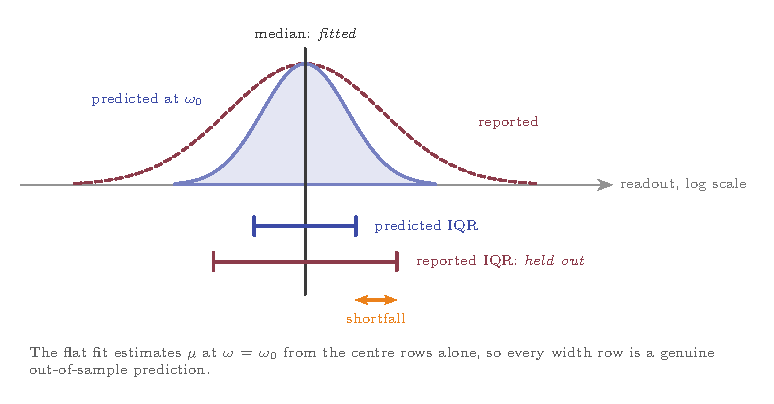
\includegraphics[height=0.62\textheight]{width_shortfall.pdf}
  \end{center}
  \undercap{A reported quartile is a width row too. Fitting $\hat q_{0.25}$ and
    $\hat q_{0.75}$ would leave the comparison measuring a residual from a fit
    that had already seen it.}
\end{frame}

\begin{frame}[t]{What the flat fit buys, and what it cannot test}
  \begin{center}\small
  \begin{tabularx}{\textwidth}{@{}lX@{}}
    \toprule
    $V_B$ is computable & The bootstrap resamples a real cloud. \\
    Width rows are held out & Predict them at $\omega_0$ and report the ratio per readout. \\
    $\hat\mu$ needs no conversion & It is already the centre of a population, so nothing has to be adjusted afterwards. \\
    It supplies the plug-in & $\phi_0=(\hat\mu_{\text{flat}},\omega_0)$. \\
    \bottomrule
  \end{tabularx}
  \end{center}
  \vfill
  \textbf{It cannot test the shape of the population}: $\omega$, $R$, and the
  direction $s$ and $b_1$ share.
\end{frame}

% ---------------------------------------------------------------- identifiability
\begin{frame}[t]{Most of $\phi$ is not identified. Which parts moved?}
  $\phi$ has far more coordinates than there are rows, so most of the posterior
  is the stage-1 prior handed straight back. That is the design rather than a
  failure. What is worth knowing is which directions the rows actually moved.
  \[
    G = I + J\Tr J,
    \qquad J = V^{-1/2}\,\frac{\partial\tau}{\partial\phi}\,\Sigma_\phi^{1/2} .
  \]
  $J$ is how much each predicted row moves when each parameter moves, put on a
  common scale: divided by that row's error bar, multiplied by that parameter's
  prior width. $G$ is then the posterior precision, and the $I$ is what the prior
  on its own would give.
  \begin{itemize}
    \item $J$ has only $K$ rows, so at least $\dim\phi-K$ directions have
      $Jv=0$. Move along one of those and not a single prediction changes, so
      the posterior there is exactly the prior.
    \item Report the eigenvalues of $G$, and how $\mathrm{tr}(J\Tr J)$ splits
      across the blocks of $\phi$.
  \end{itemize}
\end{frame}

\begin{frame}[t]{Two consequences of the shape alone}
  \begin{itemize}\setlength\itemsep{12pt}
    \item \textbf{The measurement map takes most of the information.} $a$ has a
      handful of coefficients against hundreds of mechanism parameters, and acts
      directly on the rows where the mechanism must act through the simulator.
      So whatever the model can route into $a$ will end up there, the emulator's
      offset included.
    \item \textbf{Row space is saturated.} When $\mathrm{rank}(J)$ equals the
      number of rows, ``can the model produce this row effect'' is answered yes
      by construction. A useful check therefore has to ask what an effect costs,
      not whether it is reachable.
  \end{itemize}
\end{frame}

\begin{frame}[t]{Check: can the map hold the emulator's offset?}
  To first order $a$ shifts the location rows and $b$ the scale rows. Stack those
  effects into $W$: that is everything the measurement map is able to do to the
  data. Now ask how much of the emulator's average error $\bar d$ lies inside
  that span, measured in error-bar units:
  \[
    \text{captured} = \big\|P_{V^{-1/2}W}\,V^{-1/2}\bar d\big\|
      \Big/ \big\|V^{-1/2}\bar d\big\| .
  \]
  \vfill
  A high fraction says the emulator's bias is representable, and is being paid
  for in $a$. A low one says it is sitting in $\mu$ instead.
\end{frame}

\begin{frame}[t]{Check: does $Z$ have work of its own?}
  The model claims assay modality and quantity type have no mechanistic twin.
  The obvious test, whether the mechanism could reproduce a column of $Z$, says
  yes every time: with hundreds of parameters against tens of rows the mechanism
  can hit any row pattern at all. So ask what it would \emph{cost} instead, as
  the smallest mechanism move that imitates that column:
  \[
    \delta^\ast_j = \arg\min_\delta\ \delta\Tr\Sigma^{-1}\delta
    \qquad\text{subject to}\qquad J_{\mu\omega}\,\delta = We_j .
  \]
  \vfill
  Report $\|\delta^\ast_j\|$ in prior standard deviations. Large means only an
  implausible mechanism move imitates that column, so the column is identified.
  Small means the two are confounded, and the priors decide the split.
\end{frame}

% ================================================================ weaknesses
\begin{frame}[standout]
  Where I am least sure
\end{frame}

\begin{frame}[t]{What the fixed cloud has that we do not}
  Weight collapse is at least a joint signal. One weight vector has to satisfy
  every observable at once, so what strain it shows reflects the \emph{coupling}
  between observables. A parametric fit always returns something, and has no
  equivalent of its own.
  \vfill
  \textbf{A hybrid.} Reweight the fitted $F(\theta\mid\hat\phi)$ rather than a
  wide prior. Starting from a population the data already agree with removes
  most of the collapse that dimension alone causes, so the strain that remains
  is attributable, and \alert{measures how much shape the lognormal missed}.
\end{frame}

\begin{frame}[t]{Known simplifications}
  \begin{itemize}\setlength\itemsep{8pt}
    \item \textbf{Independence across blocks.} Shared patients are handled inside
      a block, so what remains is that no two publications overlap, which
      registry sources do not guarantee.
    \item \textbf{The study offset is shrunk, not free.} $\tau_\eta$ is asserted,
      and only 7 of the 17 (quantity type, assay modality) cells are reported by
      more than one study, so the corpus constrains it weakly. Report the fit at
      more than one $\tau_\eta$.
    \item \textbf{$V$ frozen at $\phi_0$.} Letting it move with $\phi$ brings
      back a $-\tfrac12\log\det V$ term that rewards a narrow population whether
      or not it fits. The cost is that the error bars do not track $\phi$.
    \item \textbf{$Z$ is asserted, not tested.} The cost computation above is the
      version that survives the dimensions, and it has not been run.
  \end{itemize}
\end{frame}

\begin{frame}[t]{$R$ is an input, and it reaches $\omega$}
  The factor form makes $R$ cheap to state and positive definite by construction,
  but nothing pins the loadings and $R$ carries no uncertainty. Joint and tail
  questions rest on it entirely.
  \vfill
  It reaches the marginals too. Correlated parameters pushing a readout the same
  way inflate its variance, so a diagonal $R$ under-predicts spread and the fit
  inflates $\hat\omega$ to meet the published IQRs.
  \vfill
  Fit at both. If $\hat\omega$ barely moves, the marginal widths are safe and
  $R$ touches only joint statements. If it moves, they are partly an artefact.
\end{frame}

\begin{frame}[t]{The one that changes the answer}
  When the fitted population comes out narrow there are two explanations, and the
  data do not separate them:
  \begin{itemize}\setlength\itemsep{6pt}
    \item the patients really are alike ($s$), or
    \item the simulator under-disperses and $\kappa$ has stretched the readouts
      to compensate ($b_1$).
  \end{itemize}
  \vfill
  \alert{Only $s$ reaches the virtual population.} $b_1$ is discarded with the
  rest of the measurement map, so the split decides the answer.
\end{frame}

\begin{frame}[t]{$s$ against $b_1$: what would break the tie}
  \begin{itemize}\setlength\itemsep{9pt}
    \item A width row responds to $b_1$ the same way whatever it measures. It
      responds to $s$ only through the parameters whose spread is not already
      known. So a readout separates the two only if its balance between those
      differs from the other readouts'.
    \item \alert{Right now no parameter has a measured spread at all}, so that
      balance is identical everywhere and nothing separates them. The priors
      $\tau_s$ and $\sigma_b$ decide the answer between them. Report the joint
      posterior of the pair so the split is at least visible.
    \item A prior on assay measurement error would break the tie, and an assay
      CV is far easier to come by than a measured between-patient width.
  \end{itemize}
\end{frame}

% ================================================================ backup
\appendix

\begin{frame}[t]{Backup: indices and dimensions}
  \begin{center}\small
  \begin{tabularx}{\textwidth}{@{}llX@{}}
    \toprule
     & Range & \\
    \midrule
    $j$ & $1,\dots,P$ & model parameters \\
    $q$ & $1,\dots,Q$ & model species \\
    $r$ & $1,\dots,M$ & readouts \\
    $s$ & $1,\dots,S$ & scenarios \\
    $c$ & $1,\dots,C$ & study cohorts; $s(c)$ is the scenario cohort $c$ was run under \\
    $k$ & $1,\dots,K_{rc}$ & statistics that cohort $c$ reports for readout $r$ \\
    $i$ & $1,\dots,N$ & simulated patients \\
    $\Rset_c$ & $\subseteq\{1,\dots,M\}$ & the readouts that cohort $c$ reports \\
    $K_c$ & $\sum_{r\in\Rset_c}K_{rc}$ & the rows that cohort $c$ contributes \\
    $B$ & $\in\Bset$ & a block: the cohorts that have to be drawn together \\
    $K_B$ & $\sum_{c\in B}K_c$ & the rows of block $B$ \\
    \bottomrule
  \end{tabularx}
  \end{center}
\end{frame}

\begin{frame}[t]{Backup: fixed inputs}
  \begin{center}\tiny
  \begin{tabularx}{\textwidth}{@{}llX@{}}
    \toprule
    & \textbf{value} & \\
    \midrule
    $\omega_0$ & --- & Spread centre, per parameter. Elicited by role. \\
    $\Lambda,\psi$ & --- & Loadings, bins $0.8/0.5/0.3$ with a sign. Communality capped at $0.81$. \\
    $R$ & --- & Population correlation, $\Lambda\Lambda\Tr+\diag(\psi^2)$. Not identified by these data. \\
    $\mu_0,\Sigma_1$ & --- & Stage-1 composite prior, log scale. \\
    $h_r$ & --- & Readout composition, including unit conversions. \\
    $Z$ & --- & Readout attributes: assay modality, quantity type. \\
    $c_{rc}$ & --- & Pivot: cohort $c$'s median of readout $r$ at $(\mu_0,\omega_0)$. \\
    $\mathcal{S}$ & --- & Species allowed a mechanism discrepancy. Default: the shared denominators. \\
    $z_{1:N}$ & --- & The latent cloud, drawn once. \\
    $w^{(c)}$ & --- & Eligibility weights, read from each paper's criterion. \\
    $h_q,h_w$ & --- & Smoothing bandwidths: the quantile kernel and the eligibility weight. \\
    $\widehat g$ & --- & The emulator, and the design it was trained on. Fixes $E_B$ and $\bar d_B$. \\
    $V_B$ & --- & Assembled at $\phi_0$, then frozen. One per block. \\
    $E_B$ & --- & Emulator error covariance on the statistics of block $B$. \\
    \midrule
    $\tau_s$ & $0.30$ & Global level of the spreads. \\
    $\tau_\omega$ & $0.085$ & Pattern across spreads. Derived: a quarter of the role ladder's narrowest gap. \\
    $\tau$ & $0.50$ & Trust in the role prior against a measured spread. \\
    $\sigma_a,\sigma_b$ & $0.50$ & Measurement discrepancy per column of $Z$. \\
    $\tau_\beta$ & $0.15$ & Mechanism discrepancy scale, fixed rather than estimated. \\
    $\tau_\eta$ & --- & Study effect scale. Fixed rather than estimated; not yet set. \\
    \bottomrule
  \end{tabularx}
  \end{center}
\end{frame}

\begin{frame}[t]{Backup: the finite-$n$ gap, in full}
  At a log-scale spread of $1$ and $n_c=9$:
  \begin{center}\small
  \begin{tabularx}{0.92\textwidth}{@{}lrX@{}}
    \toprule
    population $q_{0.25}$ & $-0.674$ & what the statistic estimates \\
    $\mathbb{E}[\hat q_{0.25}]$ & $-0.570$ & what a paper reporting nine patients prints \\
    spread matching $-0.570$ & $0.845$ & what the fit returns if it predicts the population functional \\
    \bottomrule
  \end{tabularx}
  \end{center}
  \vfill
  The gap runs inward on both sides, so a quartile pair pulls $\Omega$ down from
  both directions. It closes as $n_c$ grows, not as the predicted cloud does.
\end{frame}

\end{document}
